\documentclass{letask}

\begin{document}
\begin{titlepage}
\center % Center everything on the page
 
%----------------------------------------------------------------------------------------
%	HEADING SECTIONS
%----------------------------------------------------------------------------------------

\textsc{\LARGE Московский\\[-0.2cm]Физико-Технический Институт\\[0.1cm]\large (государственный университет)}\\[1.5cm] % Name of your university/college
\textsc{\Large Кафедра общей физики}\\[0.1cm] % Major heading such as course name
\textsc{\large Вопрос по выбору, 3 семестр}\\[0.5cm] % Minor heading such as course title

%----------------------------------------------------------------------------------------
%	TITLE SECTION
%----------------------------------------------------------------------------------------

\HRule
\\[0.4cm]
{ \huge \bfseries Связанные колебания\\[0.2cm]
магнитных стрелок}
\\[0.6cm] % Title of your document
\HRule
\\[1.5cm]


 
%----------------------------------------------------------------------------------------
%	AUTHOR SECTION
%----------------------------------------------------------------------------------------

\begin{minipage}{0.4\textwidth}
	\begin{flushleft} \large
		\textsf{Студент}
		
		Ришат \textsc{Исхаков} \\[-0.15cm]
		513 группа
	\end{flushleft}
\end{minipage}
~
\begin{minipage}{0.4\textwidth}
	\begin{flushright} \large
		\textsf{Преподаватель}
		
		Валерий Алексеевич \\[-0.15cm]
		\textsc{Данилин} % Supervisor's Name
	\end{flushright}
\end{minipage}

\begin{bottompar}
	\begin{center}
		
\includegraphics[width = 80 mm]{logo.jpg}
	\end{center}
	{\large \today}

\end{bottompar}
\vfill % Fill the rest of the page with whitespace

\end{titlepage}


\paragraph{Цель работы:} Изучение характера связанных колебаний магнитных стрелок двух расположенных рядом компасов.

\paragraph{В работе используются:} неокуб, линейка, штатив, нитки, секундомер.

\section{Описание установки}  

Две стрелки, собранные из шести магнитных шариков неокуба, подвесим на нити за середину на некотором расстоянии $l$ друг от друга так, чтобы их оси совпадали. Под осью понимается прямая, соединяющая северный и южный конец стрелки. Стрелки будут направлены по магнитному полю Земли.

Если в начальный момент времени ($t = 0$) мы отклоним первую стрелку, вторую при этом придерживая в состоянии равновесия, а затем одновременно отпустим обе стрелки, мы будем наблюдать уменьшение амплитуды колебаний первой стрелки, в то время как для второй стрелки угол отклонения от оси будет расти. В некоторый момент первая стрелка остановится, при этом вторая стрелка будет иметь амплитуду и энергию колебания первой стрелки в начальный момент. Из-за наличия сил трения колебания будут постепенно затухать, но заметно это становится после 4-5 колебаний, трением можно будет пренебречь.

Такое явление наложения двух колебаний называется биением. Система ведет себя как связанные маятники, но в данном случае в роли соединения выступает магнитное взаимодействие между двумя намагниченными стрелками.
 
\begin{wrapfigure}[10]{l}{0.3\tw}
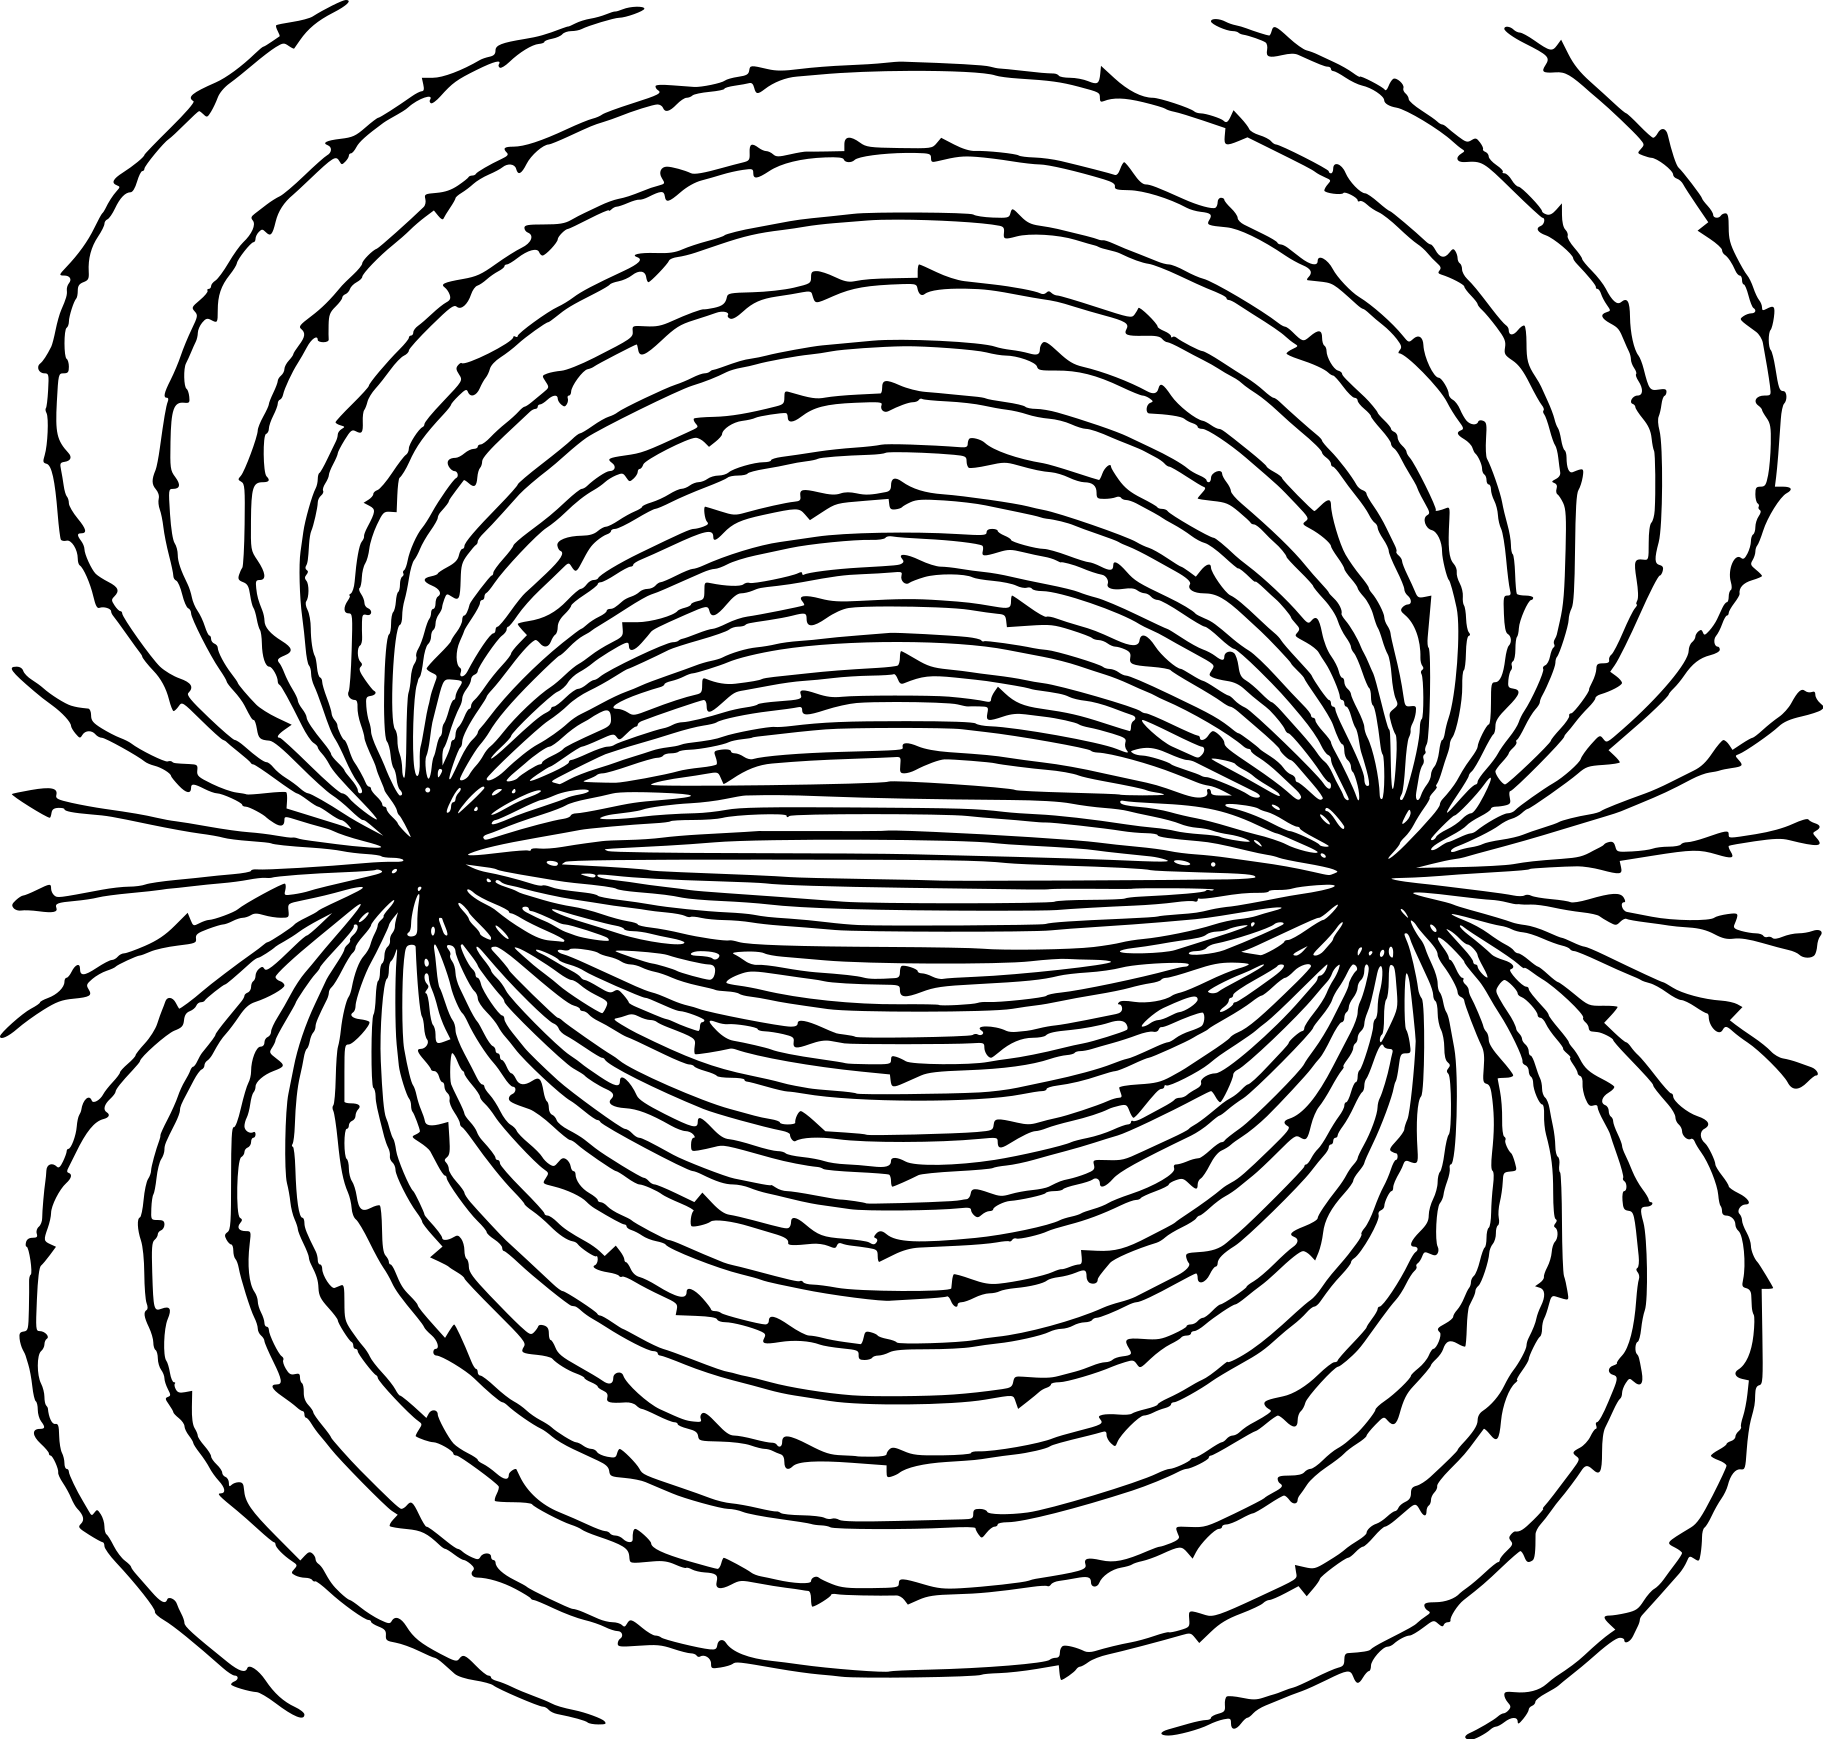
\includegraphics[width = 0.3\tw]{field}
\caption{Поле постоянного магнита}
\end{wrapfigure}

Если отклонить стрелки одновременно в одном направлении, будем наблюдать так называемые \textsf{синфазные} колебания. 
Если отклонить стрелки в разных направлениях одновременно, будем наблюдать \textsf{противофазные} колебания. 

Для объяснения природы таких колебания слегка изменим условия эксперимента: поместим стрелки так, чтобы их оси были параллельны. Так биения видно еще лучше, в связи с природой распределения магнитного поля стрелки. На конце стрелки поле более неоднородно, чем на перпендикуляре к оси стрелки в плоскости стрелки.


\section{Теория}

\subsection{Уравнение движения}  

\begin{equation}
\mathfrak{I} \cdot \vec{\varepsilon} = \vec{M},
\end{equation}
где $\mathfrak{I}$ - момент инерции стрелки относительно центра масс, $M$ - момент внешних сил.

\begin{equation}
M = \left[ \vec{p_m}, \vec{B} \right],
\end{equation}
где $\vec{p_m} = \vec{I} \cdot V$ - магнитный момент, который зависит от намагниченности $I$ и объема $V$ стрелки, $B$ - вектор магнитной индукции внешнего поля (горизонтальная компонента магнитного поля Земли)

Для малых углов $\varphi$ отклонения:

\begin{equation}
M = - p_m \cdot B \cdot \sin \varphi \approx - p_m \cdot B \cdot \varphi
\end{equation}

Дополнительный момент сил:
\begin{equation}
M_1 = p_m \cdot B_1 \cdot (\varphi_2 - \varphi_1),
\end{equation}
где $\vec{B_1}$ - вектор магнитной индукции, созданной второй стрелкой.

Так как стрелки одинаковы, то $p_m$ и $\mathfrak{I}$ для них будем считать равными. При таких условиях запишем уравнения движения обеих стрелок.

\begin{equation}
\begin{gathered}
\mathfrak{I} \ddot{\varphi_1} + p_m B \varphi_1 - p_m B_1 (\varphi_2 - \varphi_1) = 0, \\
\mathfrak{I} \ddot{\varphi_2} + p_m B \varphi_2 - p_m B_1 (\varphi_1 - \varphi_2) = 0.
\end{gathered}
\end{equation}


Сложим и вычтем уравнения, введем замену: $\alpha_1 = \varphi_1 + \varphi_2, \; \alpha_2 = \varphi_1 - \varphi_2$, получим

\begin{equation}
\begin{gathered}
\ddot{\alpha_1} + \omega_1 \alpha_1 = 0, \\
\ddot{\alpha_2} + \omega_2 \alpha_2 = 0,
\end{gathered}
\end{equation}

где $\omega_1 = \sqrt{\dfrac{p_m B}{\mathfrak{I}}}, \; \omega_2 = \sqrt{\dfrac{p_m B}{\mathfrak{I}} + 2\dfrac{p_m B_1}{\mathfrak{I}}} = \sqrt{\dfrac{p_m(B+2B_1)}{\mathfrak{I}}}$

В общем случае колебания такого магнитного маятника состоят из двух независимых колебаний с частотами $\omega_1$ и $\omega_2$, определяемые уравнениями выше и называются нормальными частотами. 

Если стрелки отклонять в одном и том же направлении на один угол, они колеблются синхронно с частотой $\omega_1$. Если же стрелки отклонить на одинаковый угол от положения равновесия в разных направлениях, тогда колебания происходят с частотой $\omega_2$.

В произвольном же случае колебаний происходят сложные колебания каждого из маятников, природа которых объясняется наличием связей.
Если считать, что $B_1 \ll B$, то есть стрелки удалены на достаточное расстояние, то можно найти связь между $\omega_1$ и $\omega_2$ ($\sqrt{1+x} \approx 1 + \dfrac{x}{2}$).

\begin{equation}
\omega_2 = \sqrt{\dfrac{p_m(B+2B_1)}{\mathfrak{I}}} = \sqrt{\dfrac{p_m B}{\mathfrak{I}}} \cdot \sqrt{1+\dfrac{2B_1}{B}} \approx \omega_1(1+\dfrac{B_1}{B})
\end{equation}

Если разность между $\omega_1$ и $\omega_2$ невелика по сравнению с самими величинами, мы видим периодическое увеличение и уменьшение амплитуды колебаний маятников. Такое явление называется биением. Их частота определяется:

\begin{equation}
\omega_{\text{б}} = \omega_2 - \omega_1 \approx \dfrac{B_1}{B} \sqrt{\dfrac{p_m B}{\mathfrak{I}}}
\end{equation}

Тогда $T_\text{б} = \dfrac{2\pi}{\omega_\text{б}}$ есть время, за которое происходит перекачка энергии.

В первом приближении $B_1 \ll B$, то есть связь слабая. Тогда поле диполя на направлении, перпендикулярном оси: $B_1 = \mu_0 \dfrac{p_m}{r^3}$.  Тогда циклическая частота биений $$\omega_\text{б} = \dfrac{B_1}{B} \sqrt{\dfrac{p_m B}{\mathfrak{I}}} \sim \dfrac{1}{r^3}$$

Однако в нашем случае положение стрелок сильно зависит от $\vec B_1$, поэтому нужно посчитать поле магнитной стрелки более строго.

\subsection{Поле магнитной стрелки при сильной связи}

Магнитные стрелки будем рассматривать как магнитные диполи. 

Поле диполя:

$$\vec{B} = \dfrac{\mu_0}{4 \pi} \left(\dfrac{3(\vec{p_m} \cdot\vec{r}) \cdot \vec{r}}{r^5} - \dfrac{\vec p_m}{r^3}\right)$$

Задача плоская, поэтому: $\vec p_m (0, 0, p_m) \; , \vec r (x, 0, z-z')$. Здесь поле в точке $(x, 0, z)$, которое создается магнитным моментом в точке $(0,0,z')$.



Разбиваем стрелку на элементарные диполи: $dp_m = \dfrac{p_m}{l} dz',$ где $l$ - длина этой стрелки.

Тогда поле элемента стрелки равно:

\begin{equation}
d \vec{B} = \dfrac{\mu_0}{4 \pi}
	\left(
		\dfrac{3 \cdot 
			\left(dp_m \cdot (z-z') \right) 
			\cdot 
			\left( \vec{i} \cdot x + \vec{k} \cdot (z-z') \right)
		}{r^5}
	- \dfrac{\vec{k} \cdot dp_m}{r^3} 
	\right)
\end{equation}

Выделим две компоненты: $dB_x$ и $dB_z$ и проинтегрируем их по всем элементам. 

%B_x
\begin{equation}
\begin{split}
B_x = \dfrac{\mu_0}{4 \pi} \bigintsss_{-\frac{l}{2}}^{\frac{l}{2}}
	\left(
		\dfrac{3 \cdot (z-z') \cdot x}
		{\left(x^2 + (z-z')^2 \right)^{\frac{5}{2}}}
	\right)&
	\dfrac{p_m}{l} dz' =
	\cdots = \\
	& = \dfrac{\mu_0}{4 \pi}
	\dfrac{x \cdot p_m}{l}
	\left(
		\dfrac{1}{\left(x^2 + (z-\frac{l}{2})^2 \right)^{\frac{3}{2}}} - 
		\dfrac{1}{\left(x^2 + (z+\frac{l}{2})^2 \right)^{\frac{3}{2}}} 
	\right)
\end{split}
\end{equation}

%B_z
\begin{equation}
\begin{split}
B_z = \dfrac{\mu_0}{4 \pi} \dfrac{p_m}{l}
\left(
	\bigintsss_{-\frac{l}{2}}^{\frac{l}{2}}
	\dfrac{3 \cdot (z-z')^2 \cdot dz'}
	{\left(x^2 + (z-z')^2 \right)^{\frac{5}{2}}} - 
	 \bigintsss_{-\frac{l}{2}}^{\frac{l}{2}}
	\dfrac{dz'} 
	{\left(x^2 + (z-z')^2 \right)^{\frac{3}{2}}}
\right) =
	\cdots = \\ 
	  = \dfrac{\mu_0}{4 \pi} \dfrac{p_m}{lx^2}
\left(
	\dfrac{\left(z+\frac{l}{2}\right)^3}
	{\left(\left(z+\frac{l}{2}\right)^2 + x^2 \right)^{\frac{3}{2}}}
\right)
\end{split}
\end{equation}

Для второй стрелки с учетом малости углов отклонения элементарный дипольный момент можно положить равным:
$$dp_m \approx \dfrac{p_m}{l} dz$$

Тогда вращательный момент, действующей со стороны первой стрелки на элемент второй стрелки:

\begin{equation}
d \vec{M} = \left[ d \vec{p_m} , \vec{B}  \right] = \vec{k} (dp_{mx} \cdot B_z - dp_{mz} \cdot B_x)
\end{equation}

$$dp_{mx} \cdot B_z = dp_m \cdot B_z \cdot \sin \varphi \approx \dfrac{p_m \cdot \varphi}{l} \cdot B_z dz$$

$$dp_{mz} \cdot B_x = dp_m \cdot B_x \cdot \cos \varphi \approx \dfrac{p_m}{l} \cdot B_x dz$$

Вычислим интегралы:

\begin{equation}
\int_{-\frac{l}{2}}^{\frac{l}{2}} B_z dz = \cdots = \dfrac{\mu_0 \cdot p_m}{2 \pi \cdot x^2}
\end{equation}

\begin{equation}
\int_{-\frac{l}{2}}^{\frac{l}{2}} B_x dz = 0
\end{equation}

Тогда вращательный момент будет:
\begin{equation}
M \approx \dfrac{\mu_0 \cdot p_m^2}{2 \pi \cdot lx^2} \cdot \varphi
\end{equation}

То есть $\omega_\text{б} \sim \dfrac{1}{r}$ при условии наличия сильной связи между магнитными стрелками.


\section{Эксперимент}
Подвесим две стрелки на нитях на различных расстояниях $r$. Будем выводить одну из стрелок из равновесия, придерживая другую. Замерим $n$ биений за некоторое время $t$. Найдем период биений $T_\text{б} = \frac{t}{n}$.

\begin{table}[H]
\centering
\resizebox{\tw}{!}{
\begin{tabular}{|c|c|c|c|c|c|c|c|c|c|c|c|c|c|c|}
\hline
$r, \, \sc \m$     & 17.5  & 19    & 20    & 22    & 23    & 24.5  & 25    & 26    & 27    & 28    & 30    & 32   & 33   & 35    \\ \hline
$t, \, \s$     & 14.35 & 12.37 & 13.23 & 14.41 & 11.28 & 16.07 & 16.72 & 13.26 & 14.13 & 15.92 & 13.68 & 7.65 & 17.4 & 20.25 \\ \hline
$n$     & 5     & 4     & 4     & 4     & 3     & 4     & 4     & 3     & 3     & 3     & 2     & 1    & 2    & 2     \\ \hline
$T_\text{б}, \s$     & 2.87  & 3.09  & 3.31  & 3.60  & 3.76  & 4.02  & 4.18  & 4.42  & 4.71  & 5.31  & 6.84  & 7.65 & 8.7  & 10.13 \\ \hline
$\ln r$ & 2.86  & 2.94  & 3.00  & 3.09  & 3.14  & 3.20  & 3.22  & 3.26  & 3.30  & 3.33  & 3.40  & 3.47 & 3.50 & 3.56  \\ \hline
$\ln T$ & 1.05  & 1.13  & 1.20  & 1.28  & 1.32  & 1.39  & 1.43  & 1.49  & 1.55  & 1.67  & 1.92  & 2.03 & 2.16 & 2.32  \\ \hline
\end{tabular}
}
\caption{Данные эксперимента}
\end{table}

Построим график $\ln T(\ln r)$, углом наклона которого будет $\alpha$ в зависимости $T = C \cdot r^{\alpha}$

\begin{figure}[H]
\centering
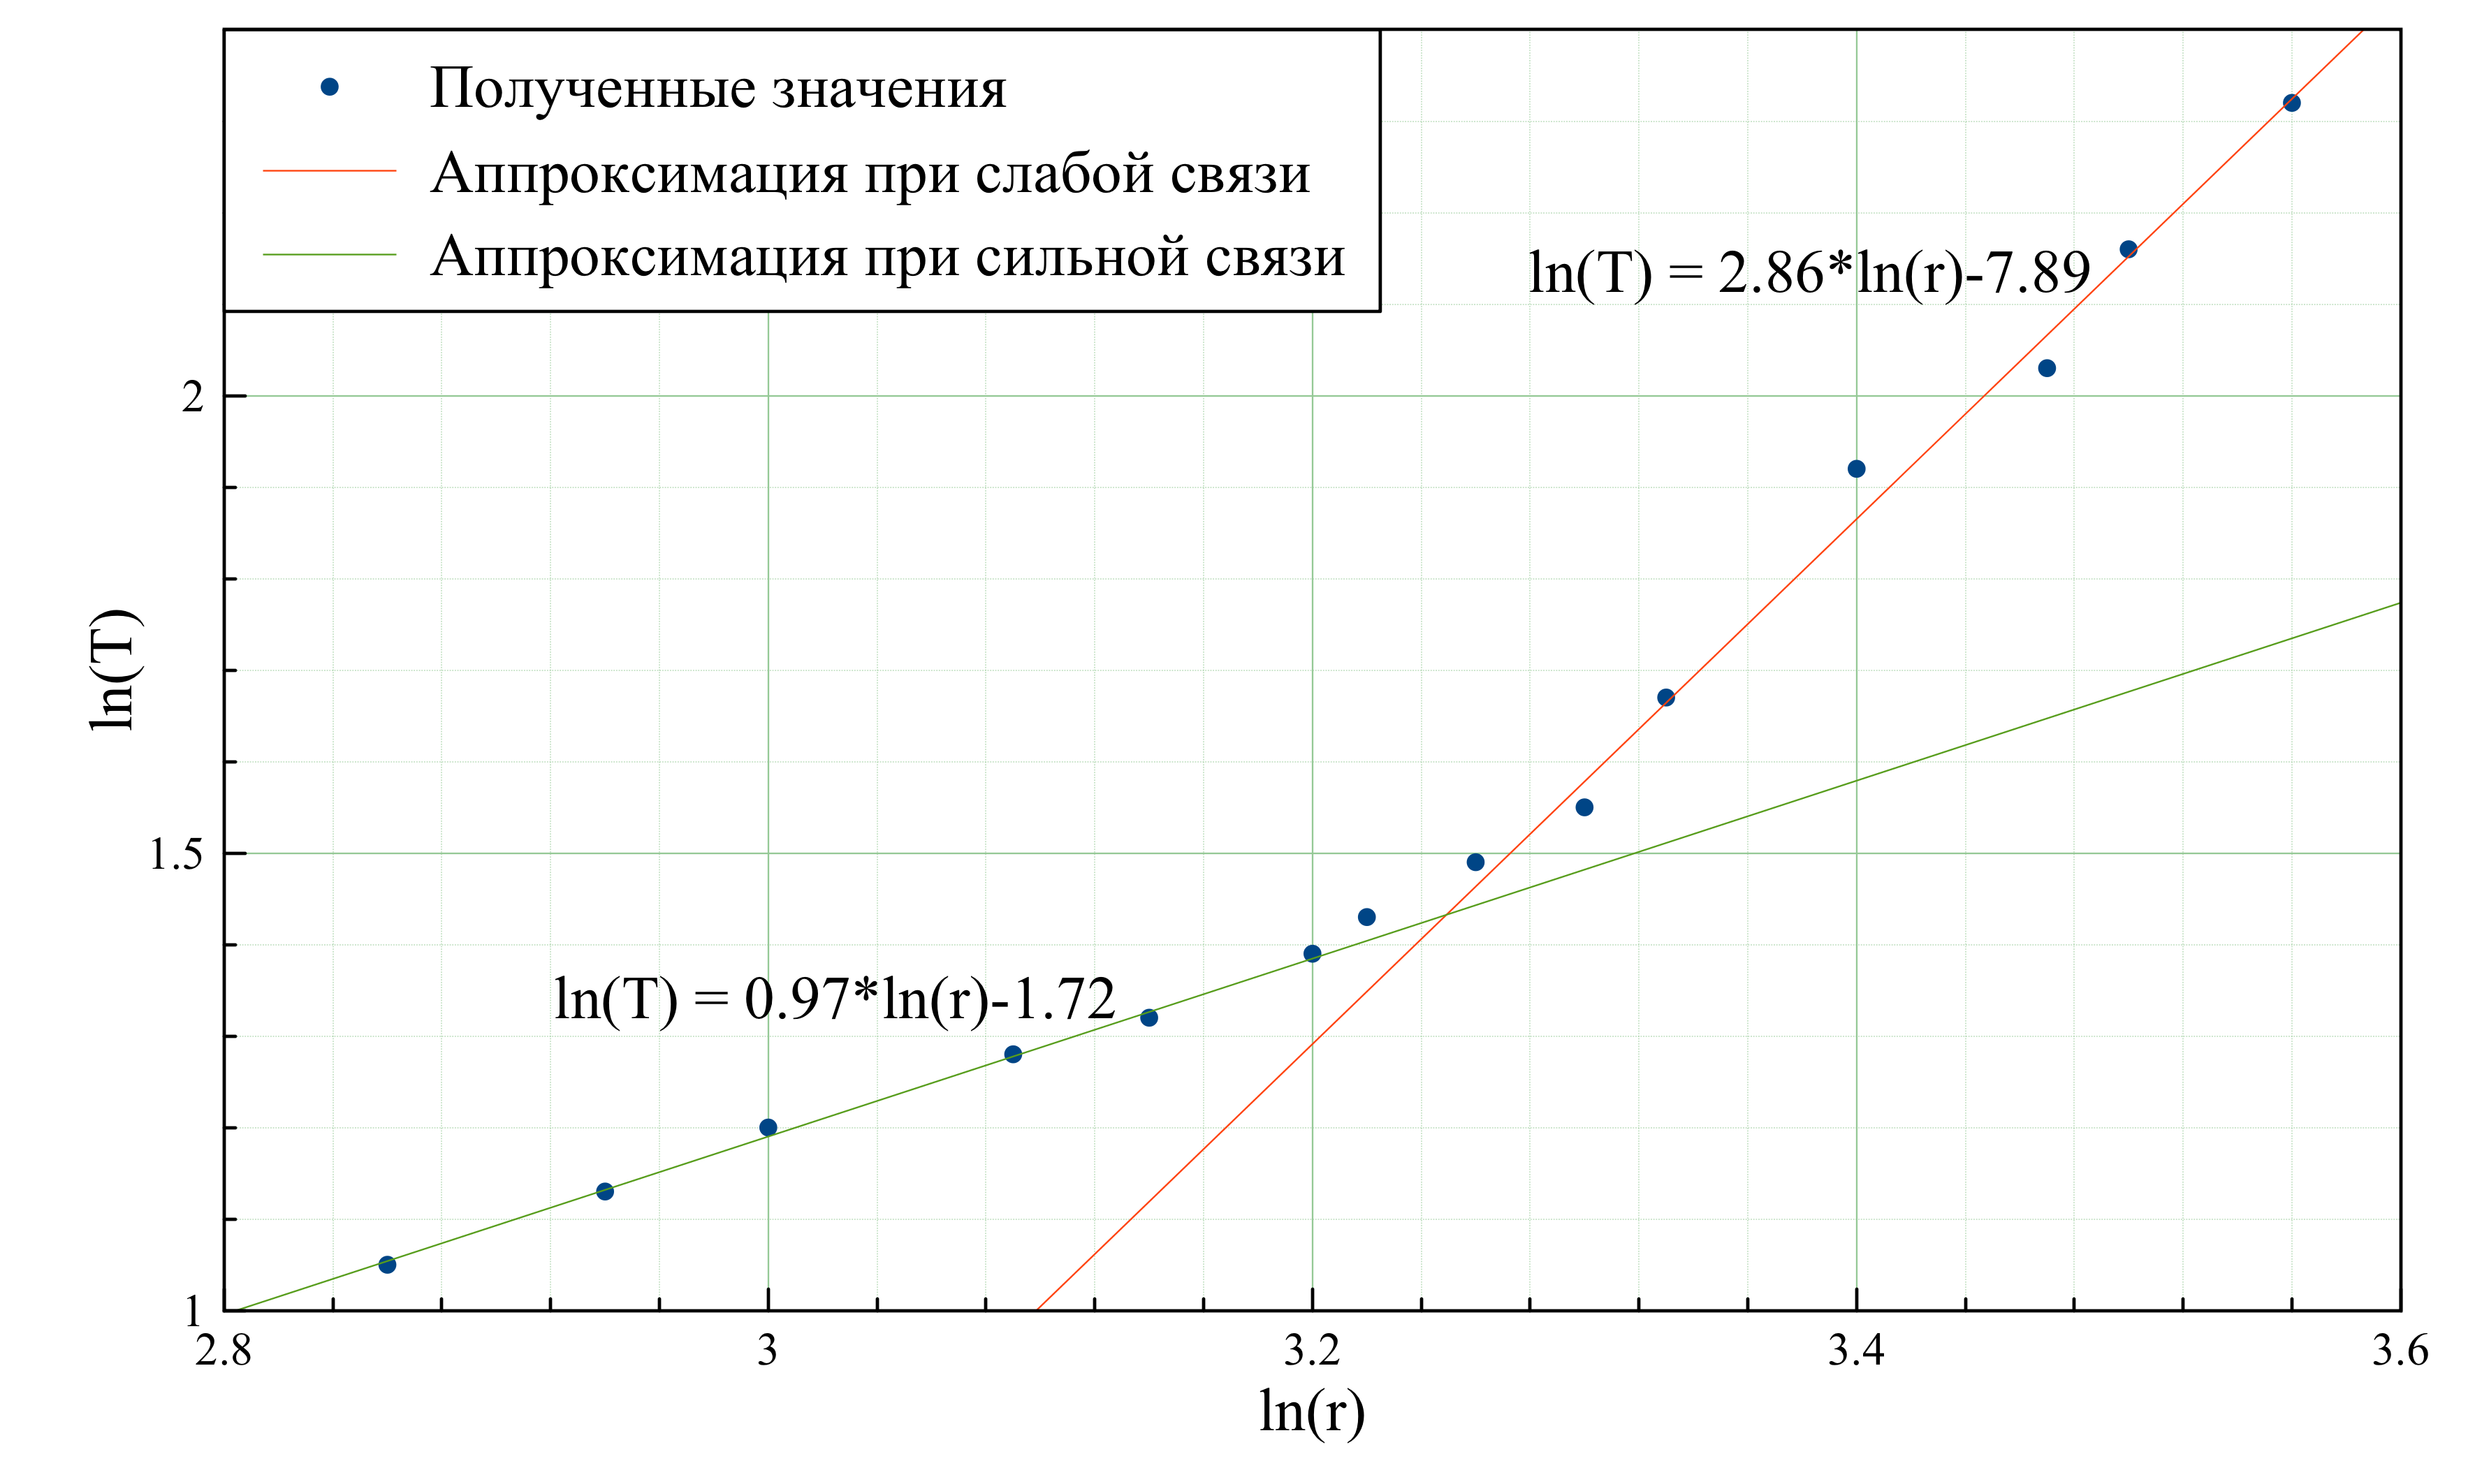
\includegraphics[width = 0.8 \tw]{Logarithmic}
\caption{Логарифмический график}
\end{figure}

\section{Вывод}  

\begin{itemize}
\item При малых расстояниях между магнитными стрелками их можно рассматривать как связанные маятники с сильной связью и наблюдать явление биения, $\omega_b \sim \dfrac{1}{r}$.

\item На больших расстояниях влияние поля стрелок друг на друга уменьшается, но биения до сих пор присутствуют с $\omega_b \sim \dfrac{1}{r^3}$.
\end{itemize}

\end{document}
